\chapter{Architecture and Design}
\section{Overview}
The application is developed and built using the Python language (v3.7.4) and it is also containerized into a Docker image which contains the Alpine Linux distribution, the operating system which runs the application using the Python language. 
The application uses a lot of geospatial libraries in Python, it also uses some libraries that were initially created in other languages (C++, Go etc), but were minimally converted to Python since they were very powerful and useful for the community.
Some of these libraries are powerful (for example the drawing library) and require a lot of dependencies which do not exist in the Alpine Linux distribution out of the box for the docker image. As a result, the docker image is not very light as it requires those dependencies first before the libraries can be used (which are necessary for the project).\\
The application mostly deals with geometry objects, API requests, correct and precise HTTP responses and some mathematical calculations for the geospatial data.\\
\newline
The docker image of this application also contains the application's libraries and some dependencies that some of those libraries use.
As soon as the docker image is built and ran, there is a command in that docker file that starts the application automatically.
\newline
\begin{figure}[H]
	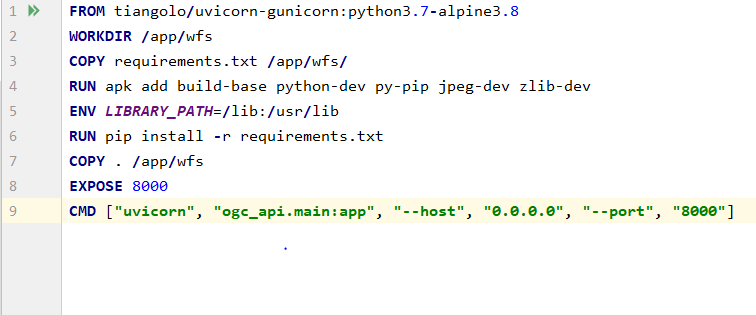
\includegraphics[width=\linewidth]{./Images/ArchitectureDesign/dockerfile_image.png}
	\caption{How the docker file looks}
\end{figure}
That docker image is then also sent to the Docker Compose tool which is a tool for defining and running docker applications (it is more suitable for multi-container applications, but works in this case too), this was added for easier accessibility, configuration and running of the container.
\newline
\begin{figure}[H]
	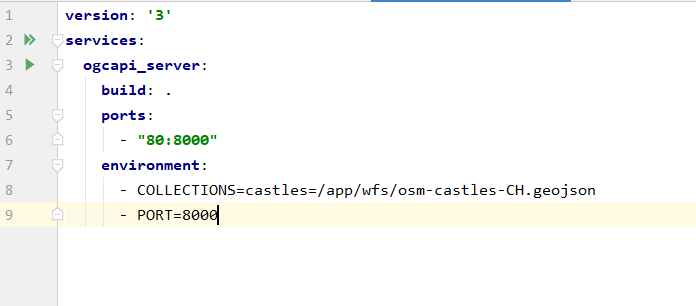
\includegraphics[width=\linewidth]{./Images/ArchitectureDesign/dockercompose_image.png}
	\caption{How the docker compose file looks}
\end{figure}
The container architecture makes it very easy to build and start the container since it only requires changing the environment variables in the docker compose (if necessary) and then running the command:
\begin{minted}{bash}
$ docker compose up --build
\end{minted}
\newpage

\section{Design Decision - Programming Language}
This application was built using the \href{https://python.org/}{Python} programming language, version 3.7.4.\\
\newline
Python is an interpreted, high-level, general-purpose programming language. Created by Guido van Rossum and first released in 1991, Python's design philosophy emphasizes code readability with its notable use of significant whitespace. Its language constructs and object-oriented approach aim to help programmers write clear, logical code for small and large-scale projects. \cite{WhatIsPython}\\
\newline
The reason why this project was chosen to be build in Python is because: it is powerful, runs everywhere, can be used in conjunction with other technologies too and has been getting a lot of attention lately.
A big difference between Python and other programming languages is the syntax and the programming paradigm it uses. Usually, when programming in Python, it requires a different way of thinking, python programmers call it a "pythonic" way of programming.\\
\newline
Here's a Python code \& syntax example for writing/reading a file:  \cite{PythonTutorialsPoint}
\begin{minted}{python}
#!/usr/bin/python

import sys

try:
# open file stream
file = open(file_name, "w")
except IOError:
print "There was an error writing to", file_name
sys.exit()
print "Enter '", file_finish,
print "' When finished"
while file_text != file_finish:
file_text = raw_input("Enter text: ")
if file_text == file_finish:
# close the file
file.close
break
file.write(file_text)
file.write("\n")
file.close()
file_name = raw_input("Enter filename: ")
if len(file_name) == 0:
print "Next time please enter something"
sys.exit()
try:
file = open(file_name, "r")
except IOError:
print "There was an error reading file"
sys.exit()
file_text = file.read()
file.close()
print file_text
\end{minted}
As you can see, this is not the typical code syntax that people write in other programming languages. However, it is very convenient and efficient once you get used to it.\\
\newpage
\section{Design Decision - Containerization}
This application is also shipped into containers, which are the new thing in the software engineering world. This project uses only one container, the application only, since that's the only required one, there is no database or front-end application which has to be separated into other containers.\\
The container architecture that this project uses is \href{https://www.docker.com/}{Docker}.\\
Docker is a set of platform as a service (PaaS) products that use OS-level virtualization to deliver software in packages called containers. Containers are isolated from one another and bundle their own software, libraries and configuration files; they can communicate with each other through well-defined channels. All containers are run by a single operating-system kernel and are thus more lightweight than virtual machines. \cite{WhatIsDocker}\\
\newline
Here's an illustration of the Docker architecture:

\begin{figure}[H]
	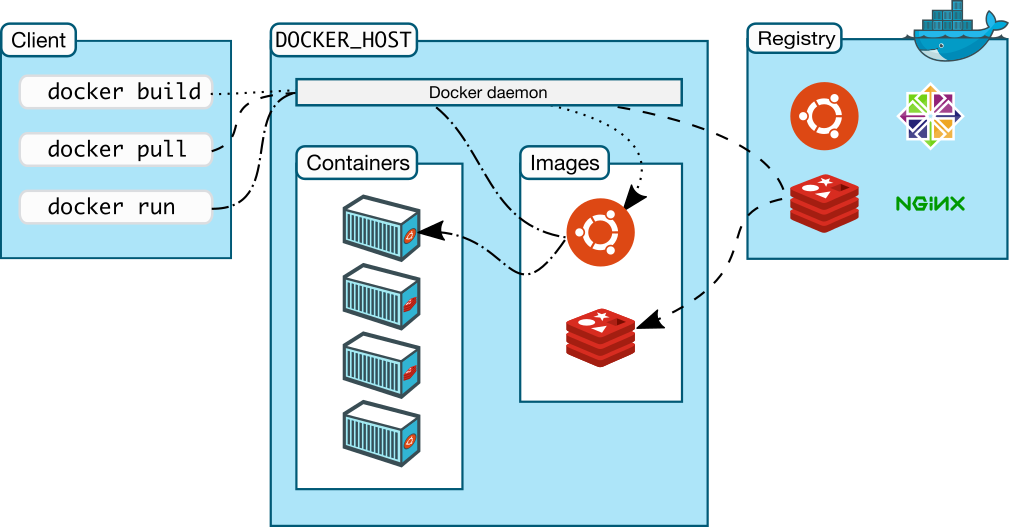
\includegraphics[width=\linewidth]{./Images/ArchitectureDesign/docker_architecture.png}
	\caption{How the docker architecture looks like \cite{DockerOverview}}
\end{figure}
\textit{Docker images} are read-only templates and can for instance contain already installed software such as Ubuntu, Python, various databases or in this case, combined image of Alpine Linux and Python. They simplify the process of creating Docker containers.

\textit{Docker registries} are used for distributing existing Docker images. They can be either private or public in the \href{https://hub.docker.com/}{Docker Hub}. Docker images are downloaded from Docker registries.

\textit{Docker containers} are built from the Docker images themselves. They contain everything needed for an application to run and have their own file system and networking.

